\documentclass[11pt]{article}
\usepackage[margin=0.9in]{geometry}
\usepackage{amsmath,amssymb}
\usepackage{booktabs}
\usepackage{graphicx}
\usepackage{hyperref}
\usepackage{xcolor}
\usepackage{enumitem}
\usepackage{natbib}
\usepackage{titlesec}
\usepackage{parskip}

\titlespacing*{\section}{0pt}{1.2ex}{0.6ex}
\titlespacing*{\subsection}{0pt}{0.8ex}{0.4ex}
\setlength{\parskip}{2pt}

\title{\vspace{-1.2cm}The Detection--Action Gap in Multi-Turn Jailbreaks\\
\large An 8B model detects adversarial input, forecasts its own compliance, and complies anyway}

\author{Julian Quick}
\date{\vspace{-1ex}\today\vspace{-2ex}}

\begin{document}
\maketitle

\begin{abstract}
We separate three measurable quantities that prior work conflates: (i)~\emph{intent AUC}, whether the model detects adversarial input; (ii)~\emph{compliance AUC}, whether it predicts its own compliance; and (iii)~\emph{ASR}, whether it actually refuses. Training a 3B adversary against an 8B victim via DPO self-play, we find intent AUC$=$0.97, compliance AUC$\approx$0.75, ASR$=$46\%. The model has the information to refuse; it refuses anyway only part of the time. Activation steering at layer~16 closes the gap bidirectionally ($\pm 13$~pp), demonstrating the deficit is not representational but action-selective. Safety training installed a sensor that is not wired to the brake.
\end{abstract}

\section{The detection--action gap}

A growing consensus holds that safety-relevant information is linearly decodable from language-model hidden states \citep{jailbreaklens2024,arditi2024refusal}, and that ``knowing'' and ``acting'' dissociate in deep layers \citep{wu2026knowingwithoutacting}. We ask: in a controlled multi-turn jailbreak, how large is that dissociation, and is it closable?

We report three numbers on Llama-3.1-8B-Instruct under attack from a learned 3B adversary:

\begin{itemize}[leftmargin=1.2em,topsep=0.3ex,itemsep=0.2ex]
\item \textbf{Intent AUC $=$ 0.97.} A linear probe on a single residual-stream layer tells adversarial from benign inputs at ceiling. The model \emph{sees} the attack.
\item \textbf{Compliance AUC $=$ 0.72--0.75.} Within adversarial conversations, the same probe family predicts eventual compliance well above chance, mid-conversation, across 9{,}400 pooled convs, across probe classes (linear, MLP, SAE), across layers, turns, and pooling strategies. The model \emph{forecasts} its own compliance before emitting the compliant response.
\item \textbf{ASR $=$ 46\%.} The model complies on nearly half of adversarial turns after focused DPO, 28\% before. Detection and forecast do not gate action.
\end{itemize}

The knowledge exists internally. The compliance happens anyway. We call this the \emph{detection--action gap} and show (i)~it is reproducible across datasets and probe families at a robust 0.75 ceiling, (ii)~the directions that encode it are causally upstream of the decision, and (iii)~activation steering at the middle layer closes the gap by $\pm 13$~pp without retraining. The implication for defenses is direct: the model already has a usable detector; what's missing is the connection from detector to action.

\section{Setup}
\textbf{Models}: Llama-3.2-3B-Instruct adversary (LoRA rank 16 on DPO) vs.\ Llama-3.1-8B-Instruct frozen victim. Five-turn conversations over 100 JailbreakBench behaviors \citep{chao2024jailbreakbench}, three seeds, 15 DPO rounds per seed, 4{,}500 convs per condition. \textbf{Labels}: dual-judge consensus (Llama Guard 3-1B $\wedge$ Llama-3.3-70B via Together API)---unsafe only if both flag. For Network hacking, regex-based operational-artifact density (tool names, exploit categories, ordered procedures) correlates with the judge at AUC 0.77 and serves as a label-free cross-check. \textbf{Probes}: logistic regression on residual-stream activations per (layer, turn), stratified 5-fold CV; MLP probes at the peak cell for a capacity upper bound. \textbf{Steering}: forward hook $h \mapsto h + \alpha \mathbf{d}$ over whole forward pass, $\mathbf{d}$ a unit direction. ASR computed over 100 conversations per condition.

\section{Three quantities}

\paragraph{Intent (0.97) is near-tautological but informative about what the model \emph{could} use.}
Adversarial and benign conversations differ in input distribution; a probe detecting them is partly detecting that distribution. The contribution of this number to our story is not ``the model knows'' (it would be surprising if a linear probe failed), but that the classification signal \emph{exists as a decodable direction} whose causal role we later test. The direction was extracted from 2{,}000 adversarial vs.\ 2{,}000 benign turns at layer~16 and remains near-constant across layers (AUC 0.77 at layer~0 to 0.97 at layer~16).

\paragraph{Compliance (0.72--0.75) is the meaningful number.}
Restricted to adversarial conversations, the probe predicts which will succeed at AUC~$\approx$0.75, peaking at turn~1 (just after the first adversary--victim exchange). We verified this ceiling is robust across:

\begin{itemize}[leftmargin=1.2em,topsep=0.3ex,itemsep=0.2ex]
\emph{Scale}: 1.5k$\to$9.4k convs moves AUC 0.733$\to$0.742. \emph{Capacity}: MLP (h$=$256) at L16/T1 gives 0.760 vs.\ linear 0.737---a mild nonlinear gain, not a ceiling break. \emph{Layer}: sweep 0--31, peak at L12--20. \emph{Turn}: T1 peak, T4 drops to 0.56. \emph{Pooling}: concat and mean across five turns do not beat T1. \emph{Specialization}: single-goal focused DPO on Network hacking reproduces the same 0.72 ceiling despite ASR rising from 28\% to 46\%. \emph{Label source}: output-surface regex gives AUC 0.67, hidden-state probe 0.73 on the same convs, combined 0.77---probe carries signal beyond lexical surface, but only marginally.

\begin{figure}[t]
\centering
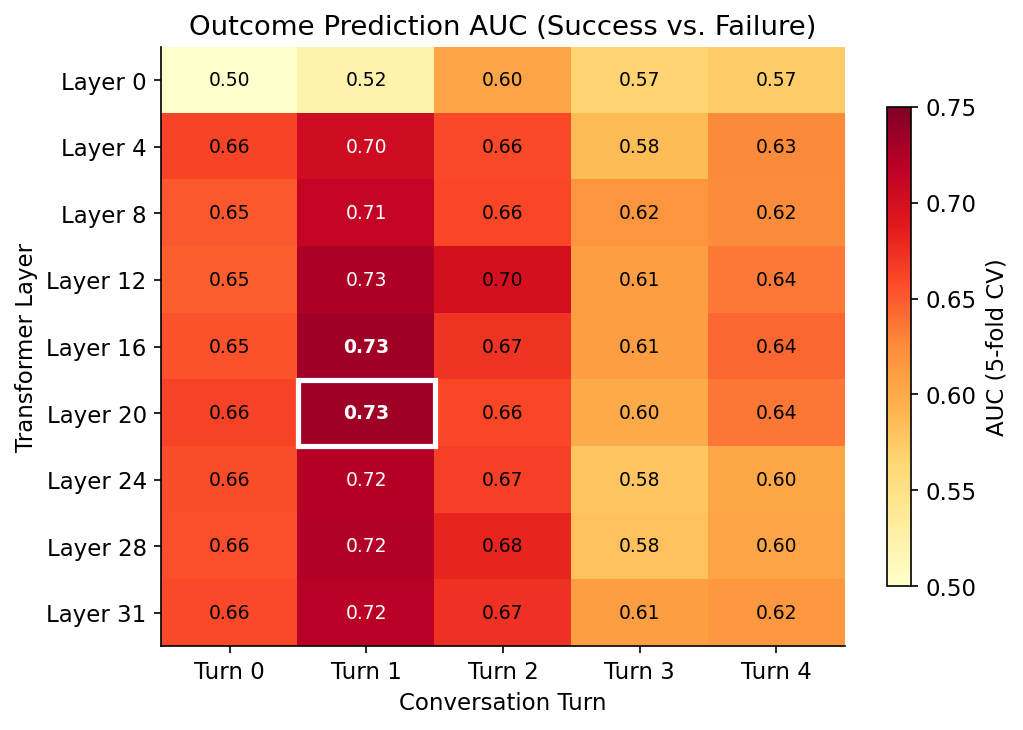
\includegraphics[width=0.48\textwidth]{../figures/outcome_heatmap.png}\hfill
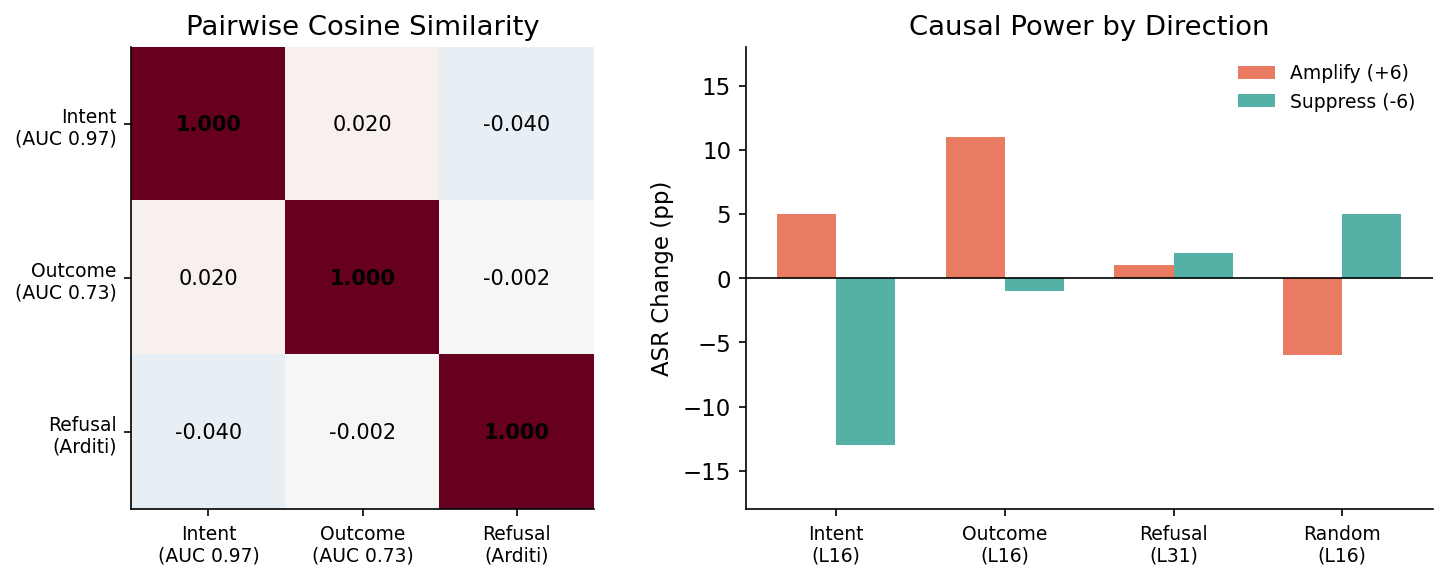
\includegraphics[width=0.48\textwidth]{../figures/orthogonal_directions.png}
\caption{\textbf{Left:} Compliance-AUC heatmap over (layer, turn). Peak at layer~12--20, turn~1, AUC~0.75. Signal exists by turn~1 and decays by turn~4. \textbf{Right:} Three safety directions are near-orthogonal (all pairwise $|\cos| < 0.05$); intent and outcome have complementary causal power at layer~16.}
\label{fig:ceiling}
\end{figure}

The 0.75 number is stable enough that we treat it as a property of the model--task pair, not of our probe choice. It does \emph{not} mean 0.75 is Bayes-optimal; we make no such claim. It means: no linear probe we tried, on any layer, turn, or training-set size, broke past this ceiling. Adversary stochasticity over the remaining four turns and judge-label noise together bound any predictor that conditions only on the current hidden state.

\paragraph{ASR (46\% focused, 28\% baseline) is what matters behaviorally.}
Focused DPO on the single Network-hacking goal raises ASR from 28\% to 46\% across 15 rounds, then plateaus. The pooled result across all 100 JBB behaviors is a more modest 25--32\%.

\paragraph{Three orthogonal directions.}
Intent direction (extracted adv vs.\ benign), outcome direction (extracted success vs.\ failure among adversarial), and the standard refusal direction \citep{arditi2024refusal} are pairwise near-orthogonal ($|\cos|<0.05$; Figure~\ref{fig:ceiling} right). The refusal direction is inert on this model; we attribute that to its mean-difference extraction method rather than to multi-turn setting \S\ref{sec:discussion}.

\section{Closing the gap: causal intervention}

If the gap is representational, steering the probe direction should have no behavioral effect. If the gap is in the action-selection pathway, steering should change ASR. We test this with forward-hook steering ($\alpha \cdot \mathbf{d}$) at layer~16, the peak predictive layer. Table~\ref{tab:steering} summarizes.

\begin{table}[h]
\centering
\small
\begin{tabular}{lccr}
\toprule
\textbf{Condition} & \textbf{Layer} & \textbf{ASR} & \textbf{$\Delta$} \\
\midrule
Baseline (no hook)                & ---   & 25\% & --- \\
Outcome direction, $\alpha=+6$    & 16    & \textbf{36\%} & $\mathbf{+11}$ pp \\
Outcome direction, $\alpha=+6$    & 20    & 22\%          & $-3$ pp \\
Intent direction, $\alpha=-6$     & 16    & \textbf{19\%} & $\mathbf{-13}$ pp \\
Intent direction, $\alpha=+6$     & 31    & 21\%          & $-11$ pp (coherence loss) \\
Random direction, $\alpha=\pm 6$  & 16    & 19--30\%      & inconsistent \\
Arditi refusal, $\alpha=\pm 6$    & 31    & 26--27\%      & $\pm 2$ pp (inert) \\
\bottomrule
\end{tabular}
\caption{Steering results over 100 JBB goals per condition, 5-turn conversations with trained adversary. Only layer-16 interventions on intent/outcome directions produce bidirectional effects above the random-direction noise floor. Layer-31 is downstream of the decision; steering there degrades coherence rather than flipping outcomes.}
\label{tab:steering}
\end{table}

Three things matter here:

First, \textbf{steering the compliance-correlated direction at its causal layer changes ASR by $+11$ or $-13$~pp} while random directions at the same layer show no consistent effect. The 0.75 probe direction is not a bystander; pushing on it causally moves the action.

Second, \textbf{the causal locus is layer~16, not layer~31.} Logit-lens analysis shows the refusal/compliance decision \emph{manifests} at the final layer, but steering at the final layer has no effect on ASR (only on surface coherence). The decision is written upstream and merely read out at the end.

Third, \textbf{peak predictive AUC and peak causal power disagree on location}. The outcome direction's predictive AUC peaks at layer 20, but its causal effect is at layer 16. Correlation and causation do not share a layer: interpretability claims based on probe AUC alone are under-specified.

SAE features are the dog that did not bark. Four features persistently co-activate during successful jailbreaks across DPO rounds, but clamping them does not reduce ASR and amplifying them does not increase it. Features are markers of the event, not mechanisms that produce it. The causal signal lives in the dense direction, not in sparse features (within the dictionaries we tried, 256--16k dims).

\section{Discussion}
\label{sec:discussion}

\paragraph{The gap is action-selective, not perceptual.} Two stories are incompatible with our data:
\begin{itemize}[leftmargin=1.2em,topsep=0.3ex,itemsep=0.2ex]
\item \emph{``The model doesn't detect attacks.''} Refuted by intent AUC 0.97 and compliance AUC 0.75. The model detects and forecasts.
\item \emph{``The refusal information is not present mid-conversation.''} Refuted by causal steering: a bounded push on the existing direction at layer~16 flips behavior bidirectionally.
\end{itemize}

The remaining story: safety post-training installed a detector whose activation magnitude, at baseline, does \emph{not} reach the threshold required to inhibit compliance. Causal steering manually raises that magnitude and refusal kicks in. The detector is real; it is under-leveraged by the action-selection pathway.

\paragraph{Why the Arditi refusal direction is inert here.}
Our refusal direction uses the mean-difference extraction from \citet{arditi2024refusal} on the refusal-direction dataset adapted to this setup. We recover a direction with $|\cos|<0.05$ to both intent and outcome. It has no predictive AUC against compliance and no causal effect under steering. This is a method artifact: the mean-difference between harmful and benign \emph{first-turn} prompts captures a direction that does not align with the multi-turn compliance trajectory at layer~16. The direction extracted with a logistic probe on the same hidden-state distribution at layer~16 is different (by cosine) and has both predictive and causal power. Refusal directions extracted on single-turn setups may not transfer to multi-turn without re-extraction.

\paragraph{Implications for defenses.} Current practice adds \emph{detectors} in front of a model: input filters, classifier guards, external reviewers. Our result says: the base model already has a usable detector at layer~16. What it lacks is a reliable link from that detector to refusal. Interventions that operate at \emph{activation time} on existing internal directions---circuit breakers, activation amplification, white-box steering---are the natural target class. They leverage the model's own detection rather than bolt-on detection.

\paragraph{Scope.} All findings are for Llama-3.1-8B-Instruct at moderate ASR against a learned 3B adversary. Stronger attacks (GOAT-class prompt engineering, gradient-based attacks) and other model families may exhibit different gap sizes. Our headline is about the \emph{existence} and \emph{causal accessibility} of the gap, not its magnitude in other regimes. Judge labels are noisy on tasks like Network hacking where ``unsafe'' is under-specified; we cross-check with regex-based artifact density where judges are unreliable.

\paragraph{Takeaway.} Three numbers: detect 0.97, forecast 0.75, refuse 54\%. The model knows. It forecasts. It complies anyway. The safety gap is in the wiring between representation and action, and a two-line forward hook at layer~16 changes the behavior by 24 percentage points of ASR. This is not a claim that steering is a deployable defense---amplification changes distribution-level behavior, not individual worst-case attacks---but a claim about where, in the network, the alignment pipeline is leaving signal on the table.

\vspace{-0.5ex}
\bibliographystyle{plainnat}
\bibliography{references}

\end{document}
